\section{Matlab}

Til dette projekt benyttes Matlab som regnemaskine og AlgoFlex som realtidsscript (mere om AlgoFlex i afsnit \ref{sec:AlgoFlex}) for at modellere en digital realtidsoplevelse af 3D-lyd. Der er lavet en GUI v.h.a. matlabs 'Guide'-funktion, som vist på figur \ref{fig:gui} hvorfra man styrer lydkildens position. Når man trykker "Play", afspilles den valgte sang i et loop, og trykker man på "Stop", stoppes hele programmet. Når musikken spiller, kan man flytte den rundt ved at indtaste den ønskede X, Y og Z koordinat. Når man trykker på "Set Position" vil man kunne se på plottet til højre på GUI'en at det blå kryds har flyttet sig til den ønskede position ift den røde cirkel som angiver lyttepositionen. Lyttepositionen fastholdes i positionen [0,0,0] og den røde stiplede streg angiver den retning som lytterens næse peger. Man vil også kunne aflæse lydkildens azimuth, elevation og distance samt høre at lydkilden er flyttet til den ønskede position. 

\begin{figure}
	\centering
	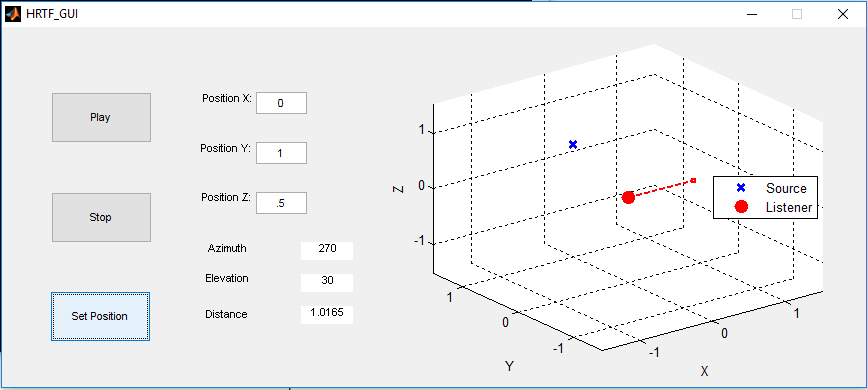
\includegraphics[width=1\linewidth]{All_Pics/GUI}
	\caption{Dette projekts grafiske brugergrænseflade til at flytte lydkilden i realtid.}
	\label{fig:gui}
\end{figure}


Lydinputtet skal være et stereosignal (eller et monosignal delt på 2 kanaler), som igennem hele 3D-rutinen modelleres hver for sig, inden de bliver afspillet i hver deres side af høretelefonerne. I scriptet er der udover et lydinput og -output, 3 modelleringer af lyden, afhængig af den ønskede azimuth, elevation og distance. \fxnote{Modellering hvordan? AB}

\subsection{Delay}

Det ønskede delay mellem de to kanaler beregnes med den udvidede pythagoræiske læresætning, hvormed man kan udregne længden af vektorer. I eksemplet fra figur \ref{fig:gui} kan afstanden $Dist_L$ fra lyttepositionens venstre øre til lydkilden beregnes som vist herunder. Lytterens hovedstørrelse $HS$ er sat til 23cm.:

\( Dist_L = \sqrt{(PosX-0)^2+(PosY-\frac{HS}{2})^2+(PosZ-0)^2}\\
 '\hspace{.9cm} = \sqrt{(0-0)^2+(1-\frac{23}{2})^2+(0.5-0)^2} = 1.0165 \)
 
 Ligeledes kan distancen til højre øre beregnes til:
 
 \( Dist_R = \sqrt{(PosX-0)^2+(PosY+\frac{HS}{2})^2+(PosZ-0)^2}\\
'\hspace{.9cm} = \sqrt{(0-0)^2+(1+\frac{23}{2})^2+(0.5-0)^2} = 1.2220 \)

Forskellen i meter er altså \( Diff_{Dist} = Dist_R - Dist_L = 0.21m \) \\
Udregner man forskellen i tid får man \( Diff_{Time} = \frac{Diff_{Dist}}{344\frac{m}{s} = 0.6ms}   \) som er den delayforskel der skal være mellem venstre og højre øre.

\subsection{Distance gain}

Distancen modelleres som nævnt ved hjælp af distancereglen, hvor der skrues 6dB op for hver halvering af distancen, og ligeledes dæmpes med 6dB når distancen fordobles. Dette udregnes ud fra lydkildens startposition, som er 1 meter foran lyttepositionen.

\subsection{HRTF}

Hvis man ville have en præcis beregning af et helt bestemt azimuth og elevation, kunne man risikere at dette punkt ville ligge mellem to (eller flere) HRTF målepunkter. Dette kunne man komme omkring ved en interpolation af de omkringliggende punkter. Dette projekt har dog haft fokus på realtidsdelen, og derfor runder Matlab-algoritmen automatisk op eller ned til nærmeste tilgængelige HRTF-data. Med disse data importeres den rigtige impulsrespons til hvert øre, og foldes på musiksignalet.